% GC-SDOH-28 Caregiver-Specific Social Determinants Instrument
% Requires packages: tikz, xcolor

\documentclass{article}
\usepackage[margin=1in]{geometry}
\usepackage{tikz}
\usetikzlibrary{shapes.geometric, arrows, positioning, fit, calc}
\usepackage{xcolor}

% Define GiveCare color palette
\definecolor{gcOrange}{RGB}{255, 159, 28}        % #FF9F1C
\definecolor{gcLightOrange}{RGB}{255, 191, 104}  % #FFBF68
\definecolor{gcTan}{RGB}{203, 153, 126}          % #CB997E
\definecolor{gcLightPeach}{RGB}{255, 232, 214}   % #FFE8D6
\definecolor{gcDarkBrown}{RGB}{84, 52, 14}       % #54340E

\begin{document}

\begin{figure}[htbp]
\centering
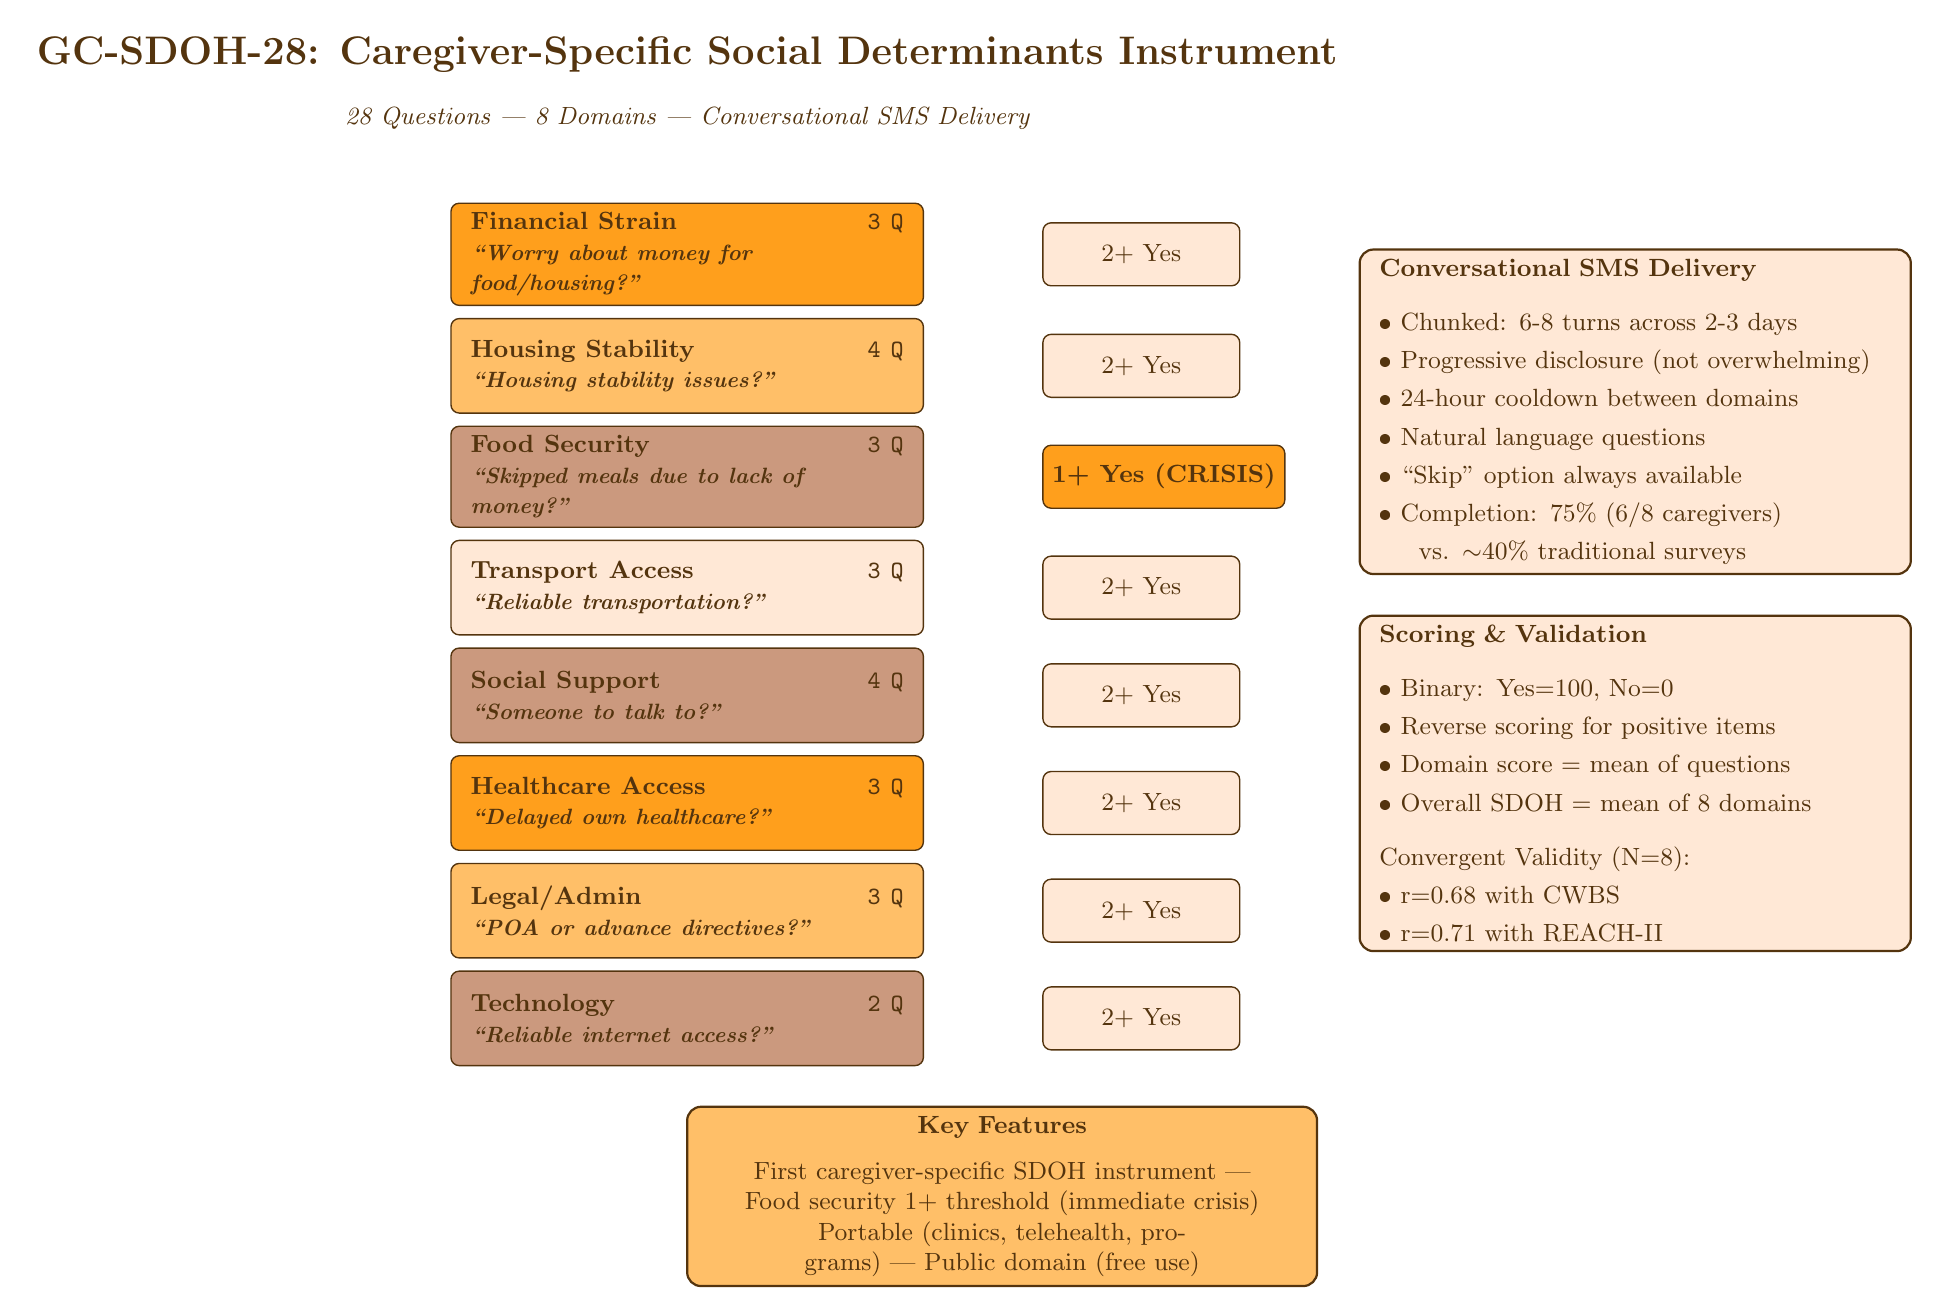
\begin{tikzpicture}[
    node distance=0.15cm,
    domainbox/.style={
        rectangle,
        rounded corners=3pt,
        minimum width=6cm,
        minimum height=1.2cm,
        text width=5.5cm,
        align=left,
        font=\small\bfseries,
        draw=gcDarkBrown,
        line width=0.5pt
    },
    response/.style={
        rectangle,
        rounded corners=3pt,
        minimum width=2.5cm,
        minimum height=0.8cm,
        text centered,
        font=\small,
        draw=gcDarkBrown,
        fill=gcLightPeach,
        line width=0.5pt
    },
    infobox/.style={
        rectangle,
        rounded corners=5pt,
        minimum width=7cm,
        minimum height=4cm,
        text width=6.5cm,
        align=left,
        font=\small,
        draw=gcDarkBrown,
        fill=gcLightPeach,
        line width=0.8pt
    },
    keybox/.style={
        rectangle,
        rounded corners=5pt,
        minimum width=8cm,
        minimum height=1.5cm,
        text width=7.5cm,
        align=center,
        font=\small,
        draw=gcDarkBrown,
        fill=gcLightOrange,
        line width=0.8pt
    }
]

% Title
\node[font=\Large\bfseries, color=gcDarkBrown] (title) at (0, 0) {GC-SDOH-28: Caregiver-Specific Social Determinants Instrument};
\node[font=\small\itshape, color=gcDarkBrown, below=0.2cm of title] (subtitle) {28 Questions | 8 Domains | Conversational SMS Delivery};

% Left column - Domains
\node[domainbox, fill=gcOrange, text=gcDarkBrown, below=0.8cm of subtitle, anchor=north] (fs) {
    Financial Strain \hfill \texttt{3 Q}\\
    \textit{\footnotesize ``Worry about money for food/housing?''}
};

\node[domainbox, fill=gcLightOrange, text=gcDarkBrown, below=of fs] (hs) {
    Housing Stability \hfill \texttt{4 Q}\\
    \textit{\footnotesize ``Housing stability issues?''}
};

\node[domainbox, fill=gcTan, text=gcDarkBrown, below=of hs] (food) {
    Food Security \hfill \texttt{3 Q}\\
    \textit{\footnotesize ``Skipped meals due to lack of money?''}
};

\node[domainbox, fill=gcLightPeach, text=gcDarkBrown, below=of food] (trans) {
    Transport Access \hfill \texttt{3 Q}\\
    \textit{\footnotesize ``Reliable transportation?''}
};

\node[domainbox, fill=gcTan, text=gcDarkBrown, below=of trans] (social) {
    Social Support \hfill \texttt{4 Q}\\
    \textit{\footnotesize ``Someone to talk to?''}
};

\node[domainbox, fill=gcOrange, text=gcDarkBrown, below=of social] (health) {
    Healthcare Access \hfill \texttt{3 Q}\\
    \textit{\footnotesize ``Delayed own healthcare?''}
};

\node[domainbox, fill=gcLightOrange, text=gcDarkBrown, below=of health] (legal) {
    Legal/Admin \hfill \texttt{3 Q}\\
    \textit{\footnotesize ``POA or advance directives?''}
};

\node[domainbox, fill=gcTan, text=gcDarkBrown, below=of legal] (tech) {
    Technology \hfill \texttt{2 Q}\\
    \textit{\footnotesize ``Reliable internet access?''}
};

% Middle column - Response options
\node[response, text=gcDarkBrown, right=1.5cm of fs] (r1) {2+ Yes};
\node[response, text=gcDarkBrown, right=1.5cm of hs] (r2) {2+ Yes};
\node[response, right=1.5cm of food, fill=gcOrange, text=gcDarkBrown] (r3) {\textbf{1+ Yes (CRISIS)}};
\node[response, text=gcDarkBrown, right=1.5cm of trans] (r4) {2+ Yes};
\node[response, text=gcDarkBrown, right=1.5cm of social] (r5) {2+ Yes};
\node[response, text=gcDarkBrown, right=1.5cm of health] (r6) {2+ Yes};
\node[response, text=gcDarkBrown, right=1.5cm of legal] (r7) {2+ Yes};
\node[response, text=gcDarkBrown, right=1.5cm of tech] (r8) {2+ Yes};

% Right column - Info boxes
\node[infobox, text=gcDarkBrown, right=1.5cm of r1, yshift=-2cm] (delivery) {
    \textbf{Conversational SMS Delivery}\\[0.3cm]
    • Chunked: 6-8 turns across 2-3 days\\[0.1cm]
    • Progressive disclosure (not overwhelming)\\[0.1cm]
    • 24-hour cooldown between domains\\[0.1cm]
    • Natural language questions\\[0.1cm]
    • ``Skip'' option always available\\[0.1cm]
    • Completion: 75\% (6/8 caregivers)\\[0.1cm]
    \hspace{0.5cm}vs. $\sim$40\% traditional surveys
};

\node[infobox, text=gcDarkBrown, below=0.5cm of delivery] (validation) {
    \textbf{Scoring \& Validation}\\[0.3cm]
    • Binary: Yes=100, No=0\\[0.1cm]
    • Reverse scoring for positive items\\[0.1cm]
    • Domain score = mean of questions\\[0.1cm]
    • Overall SDOH = mean of 8 domains\\[0.3cm]
    Convergent Validity (N=8):\\[0.1cm]
    • r=0.68 with CWBS\\[0.1cm]
    • r=0.71 with REACH-II
};

% Bottom - Key Features
\node[keybox, text=gcDarkBrown, below=0.5cm of tech, xshift=4cm] (keyfeatures) {
    \textbf{Key Features}\\[0.2cm]
    First caregiver-specific SDOH instrument | Food security 1+ threshold (immediate crisis)\\
    Portable (clinics, telehealth, programs) | Public domain (free use)
};

\end{tikzpicture}
\caption{GC-SDOH-28: A caregiver-specific social determinants of health instrument with 8 domains, conversational SMS delivery, and validated scoring.}
\label{fig:gc-sdoh-28}
\end{figure}

\end{document}
